\section*{Pr{\'e}ambule}

Voici l'{\'e}chelle que nous avons choisi pour le d{\'e}veloppement du
logiciel.
{\bf 1} signifie que la priorit{\'e} est minimale et {\bf 5} repr{\'e}sente
les fonctionnalit{\'e}s vitales au bon fonctionnement de l'application.
\begin{center}
\scalebox{1}{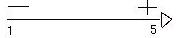
\includegraphics{images/echelle.jpg}}
\par Echelle\\
\end{center}

\par Voici les differents styles de police utilis{\'e}s : \\
{\it Italique}  : Menu contenu dans l'application.\\
{\bf Gras} 	: Titres.\\
